\newcommand{\duedatetime}{See Canvas for the due date}
% 16384_doc.cls lives in latex/ relative to this file; input@path lets
% \documentclass find it there without changing directory structure.
\makeatletter
\def\input@path{{latex/}}
\makeatother
\documentclass{16384_doc}

\newcommand{\assignmentname}{Assignment 8: DH Parameters}
\graphicspath{{latex/}}

\ifdef{\writeup}{\printanswers}

\begin{document}
\maketitle
\tableofcontents

\section{Overview}
This assignment reinforces the following topics:
\begin{itemize}

\item DH Parameters

\end{itemize}

\newpage

\section{Written Questions}
For all of the following questions, please fully compute all answers and show
your work for full credit, unless otherwise specified. Submit your answers in a
PDF entitled \verb!writeup.pdf! in your handin directory.  All answers must be
typed, but diagrams may be hand-drawn and scanned in.  However, they must be
tidy and fully legible! Consider drawing them in a black or blue pen.  All units
are in radians and meters, where appropriate.

\begin{questions}
    \titledquestion{DH Frames and Parameters}
    The RRR arm below is shown at its zero pose ($\theta_1=\theta_2=\theta_3=0$). Joint 1 turns about the vertical axis, and joints 2 and 3 turn about axes perpendicular to the page. Place the base frame (frame 0) at the bottom of the vertical column with $z_0$ up, $x_0$ to the right and $y_0$ into the page. Frame 3 is the tool frame at the end of link 3. A positive rotation of joints 2 and 3 raises the arm.
    \begin{center}
    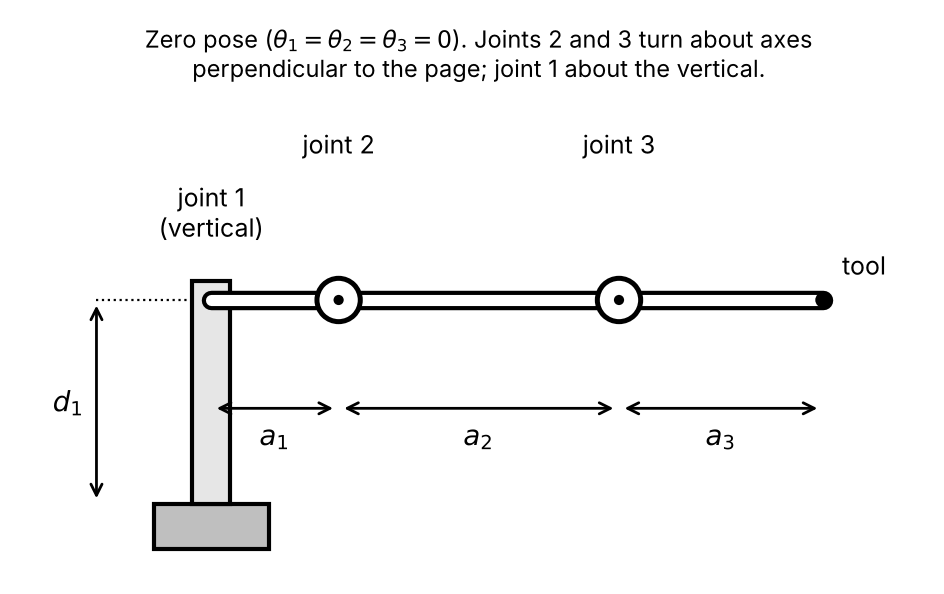
\includegraphics[width=0.85\linewidth]{figures/RRR_arm.png}
    \end{center}
    \begin{parts}
        \part[4] Using the Denavit-Hartenberg convention, state the direction ($x_i$, $y_i$, $z_i$) of frames 1, 2 and 3 at the zero pose, and where each origin is. A sketch on the figure is fine.
        \begin{tcolorbox}[height=6cm]
         % TODO: ENTER YOUR ANSWER HERE
        \end{tcolorbox}

        \part[4] Fill in the DH table ($a_i$, $\alpha_i$, $d_i$, $\theta_i$) for the arm, marking the joint variables.
        \begin{tcolorbox}[height=6cm]
         % TODO: ENTER YOUR ANSWER HERE
        \end{tcolorbox}

        \part[6] Using your table, find the position of the origin of frame 3 in the base frame as a function of $\theta_1,\theta_2,\theta_3$, and check it at the zero pose against the figure.
        \begin{tcolorbox}[height=10cm]
         % TODO: ENTER YOUR ANSWER HERE
        \end{tcolorbox}
    \end{parts}

    \newpage

    \titledquestion{Intermediate Transformations}
    Using the DH parameters below for the SCARA arm find the below homogeneous transformation matrices. 
    \begin{center}
    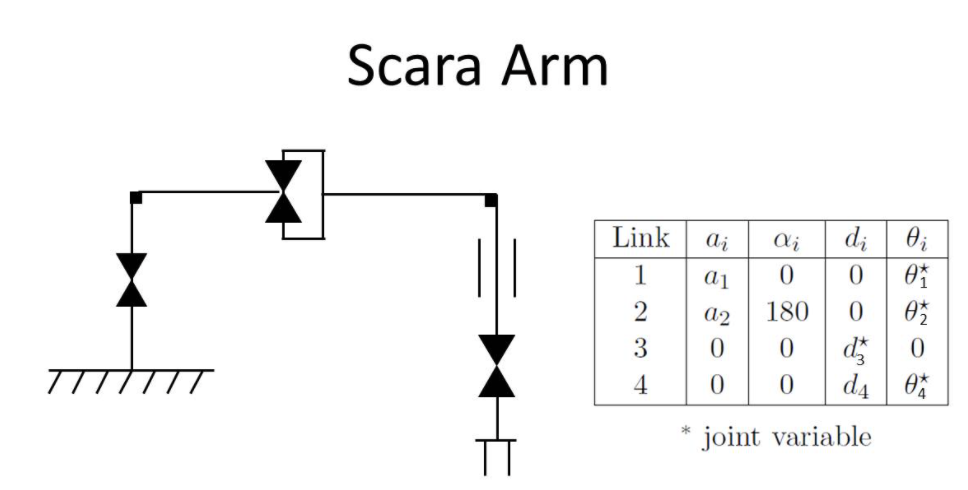
\includegraphics[width=\linewidth]{figures/SCARA.png}
    \end{center}
    \newpage
    \begin{parts}
        \part[2] $H^0_1$
        \begin{tcolorbox}[height=5cm]
         % TODO: ENTER YOUR ANSWER HERE
        \end{tcolorbox}
        
        \part[2] $H^1_2$
        \begin{tcolorbox}[height=5cm]
         % TODO: ENTER YOUR ANSWER HERE
        \end{tcolorbox}
        
        \part[2] $H^2_3$
        \begin{tcolorbox}[height=5cm]
         % TODO: ENTER YOUR ANSWER HERE
        \end{tcolorbox}
        \newpage
        \part[2] $H^3_4$
        \begin{tcolorbox}[height=5cm]
         % TODO: ENTER YOUR ANSWER HERE
        \end{tcolorbox}
    \end{parts}
    
    \titledquestion{Origin frames and Z axes}
    Calculate the Origin frames and Z axes at each joint. 
    \begin{parts}
        \part[2] Joint 1
        
        \begin{tcolorbox}[height=4cm]
         % TODO: ENTER YOUR ANSWER HERE
        \end{tcolorbox}
        
        \part[2] Joint 2
        
        \begin{tcolorbox}[height=4cm]
         % TODO: ENTER YOUR ANSWER HERE 
        \end{tcolorbox}
        
        \part[2] Joint 3
        
        \begin{tcolorbox}[height=4cm]
         % TODO: ENTER YOUR ANSWER HERE
        \end{tcolorbox}
        
        \part[2] Joint 4
        
        \begin{tcolorbox}[height=4cm]
         % TODO: ENTER YOUR ANSWER HERE
        \end{tcolorbox}
    \end{parts}
    
\end{questions}

\begin{submissionChecklist}
		\item Upload \verb!writeup.pdf! to Gradescope.
\end{submissionChecklist}

\end{document}
